\documentclass[25pt, a0paper, portrait]{tikzposter}
\usepackage[utf8]{inputenc}
 \usepackage{amsmath}% http://ctan.org/pkg/amsmath
\usepackage{natbib}
 
\usepackage{blindtext}
\usepackage{comment}
\usepackage{pifont}

\usetheme{Rays}
 
\begin{document}
% 
\
\title{ \LARGE{Simulating cryo-EM maps using a  Generative Adversarial Network (cryo-GAN)}}
%
\author{Mark Rozanov $\cdot$ Haim J. Wolfson}
\institute{Blavatnik School of Computer Science, Tel-Aviv University}
% 
%
% 
\maketitle[width=0.8\textwidth]
%\node[above right,opacity=0.9003,inner sep=0pt,outer sep=0pt] at (0,0) { 
\includegraphics[width=0.28\textwidth]{logoTA.jpg}};

\block{Abstract}{    The ability to perform a realistic simulation of a cryo-EM density map (at appropriate resolution) is crucial for the development and analysis of advanced cryo-EM based macromolecular structure modeling algorithms. In particular, such simulation is required for the recent machine learning based algorithms, which have to be trained on very large databases of "realistic" data.  Such large databases are currently unavailable, and thus have to be simulated.   
The currently used simulation methods, such as pdb2mrc from the Chimera package, usually perform averaging on atomic resolution structures from the PDB.   It is well known, that the resulting simulative structures (at the appropriate resolution) are significantly more similar to the atomic resolution structures than experimental cryo-EM maps at the same resolution, and thus do not represent the same degree of difficulty for the tested algorithms.
Cryo-GAN exploits recent deep learning techniques for creating cryo-EM maps which are indistinguishable from experimental ones. It uses the VAE-GAN architecture which is a compound Generative Adversarial Network (GAN) with Variation AutoEncoder (VAE).  Both are proven deep learning techniques for generating 2D and 3D images.
The resulting synthetic maps have a high resemblance to the experimental maps. An independent discriminator was trained to distinguish between experimental and synthetic maps. In our computational experiments the discriminator marks all voxels of a map generated by existing simulation (pdb2mrc) as non-real. Less than half of the voxels of a map generated by Cryo-GAN are marked as non-real, meaning the map is indistinguishable from an experimental one.}
 
\begin{columns}
    \column{0.6}
    \block{1. Motivation: When a simulation is required}{ Bla}
 
    \column{0.4}
    \block{2. Current Method: \\  pdb2mrc from EMAN \cite{Ludtke1999}}{{\Large

\begin{center}
\begin{tabular}{ |c|c|c| } 
 \hline
   & pdb2mrc & real map \\ 
   \hline
 represents an ”ideal” universe & \ding{52} & \ding{55} \\ 
 \hline
 contains experimental inaccuracies & & \\and real-world noise  & \ding{55} &  \ding{52} \\
 \hline
 affected by physico-chemical properties & & \\ such as charge, bonds &
  \ding{55} &  \ding{52} \\ 
 
 \hline
\end{tabular}
\end{center}
} }
\end{columns}

\begin{columns}
   \column{0.5}
\block{3. Generating a  Realistic Map -\\ use VAE \cite{Larsen2016}  Neural Network }
{        \begin{tikzfigure}
           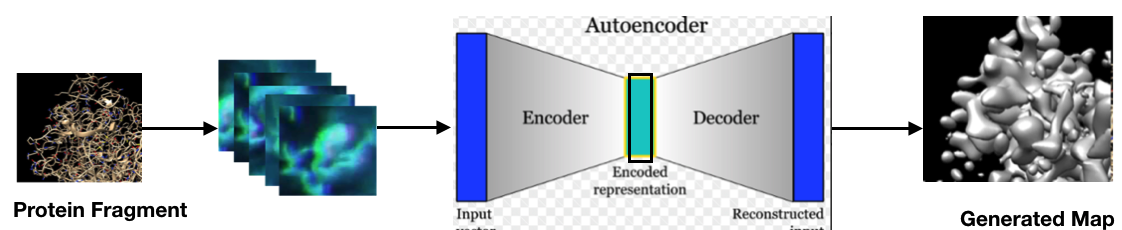
\includegraphics[width=0.45\textwidth]{VAE.png}
        \end{tikzfigure}
\textbf{Input:} Protein Structure Fragment after Voxelization; 
\textbf{Output:} 3D cryo-EM map}
   \column{0.5}
    \block{4. Make more Realistic - Adversarial Approach \cite{Goodfellow2016}}{         \begin{tikzfigure}
           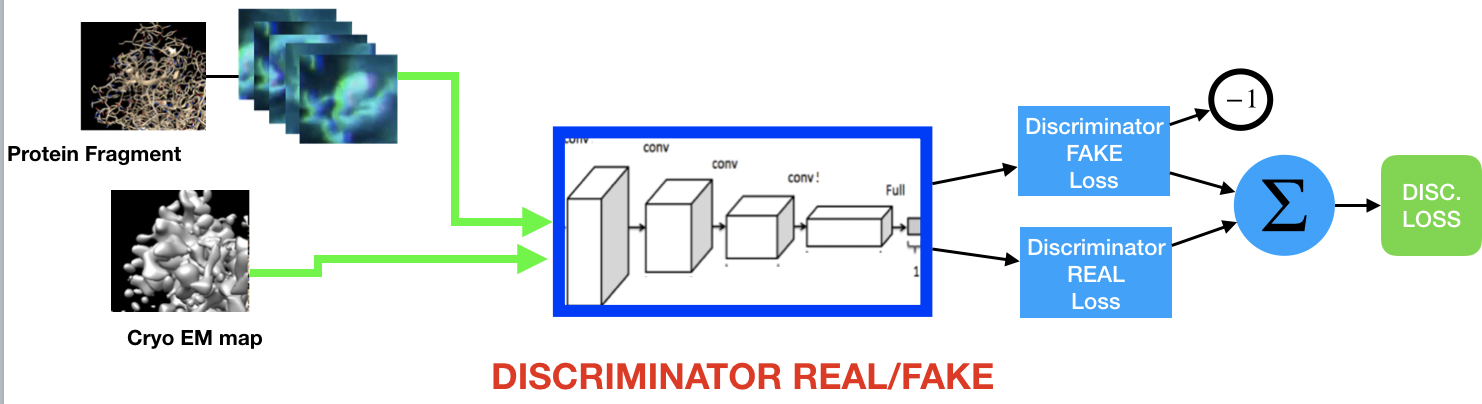
\includegraphics[width=0.45\textwidth]{gan.png}
        \end{tikzfigure}
The role of a \textbf{discriminator} is to distinguish between real (input) and fake (generated) map.}
\end{columns}
%
 

\begin{columns}
    \column{0.7}
    \block{6. Results: cryoEM map of STING protein (pdb ID 6nt8) }
    {	
    		\begin{minipage}{0.209\textwidth}
{\Large Existing Simulation - pdb2mrc}
        \begin{tikzfigure}
           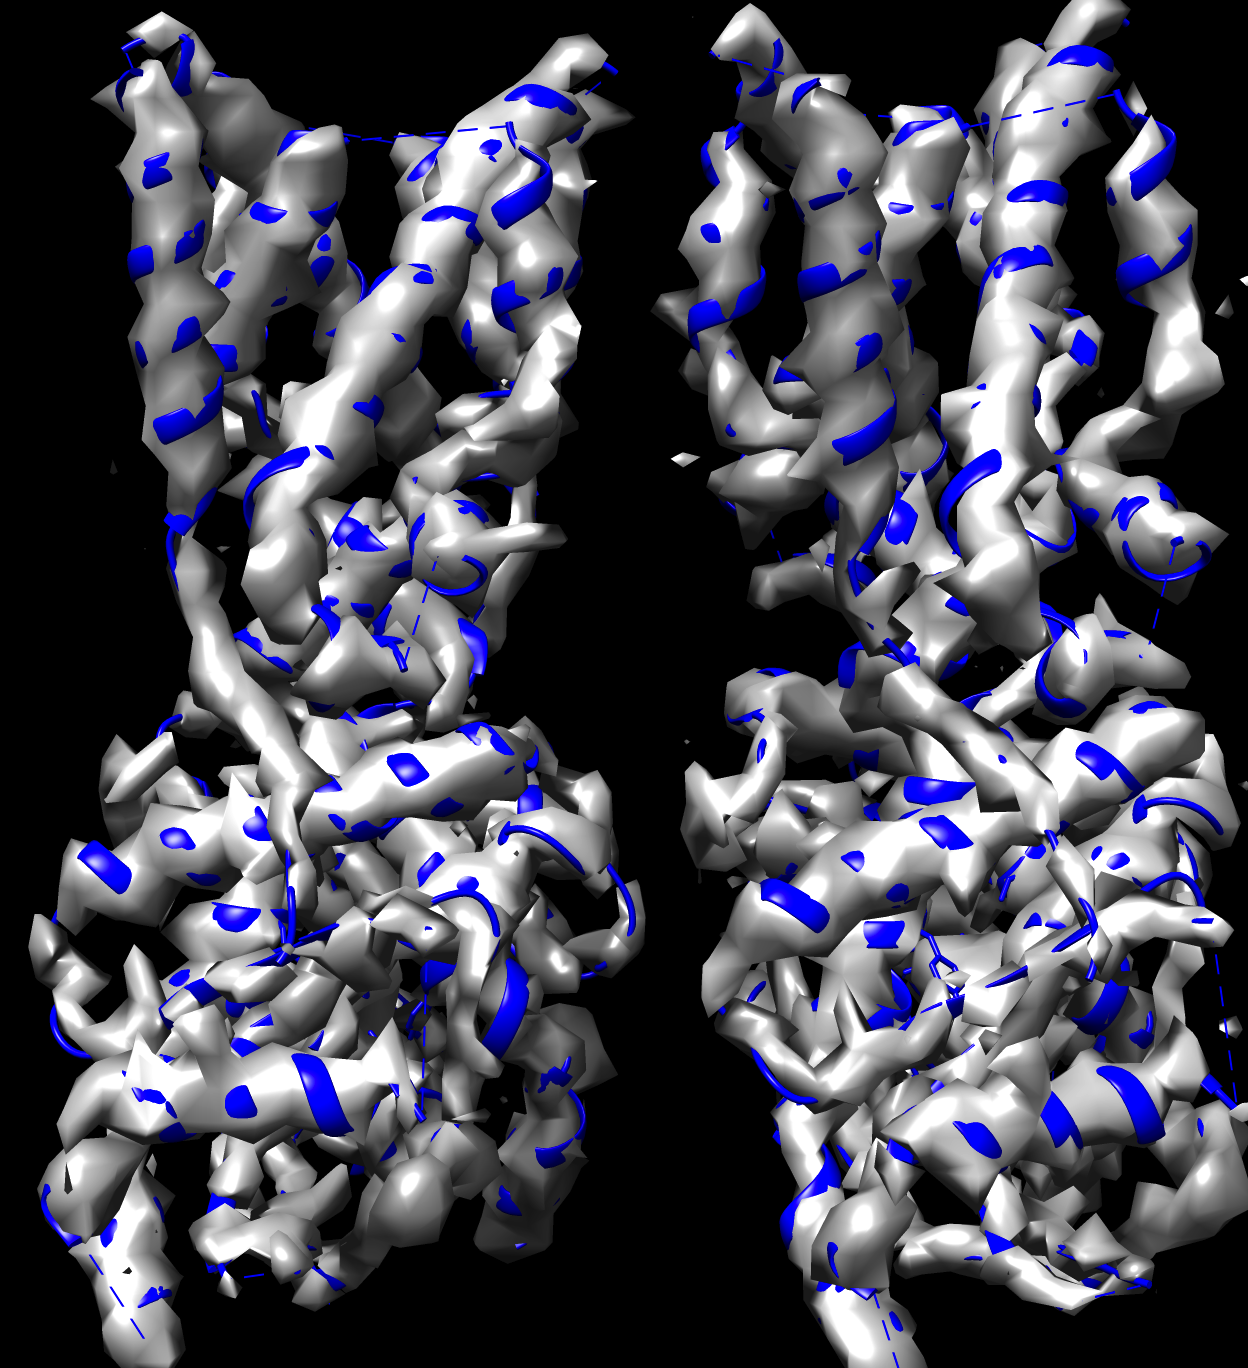
\includegraphics[width=0.9\textwidth]{mol_map.png}
        \end{tikzfigure}
\end{minipage}
\begin{minipage}{0.209\textwidth}
{\Large Real Map - EMD0505}
        \begin{tikzfigure}
           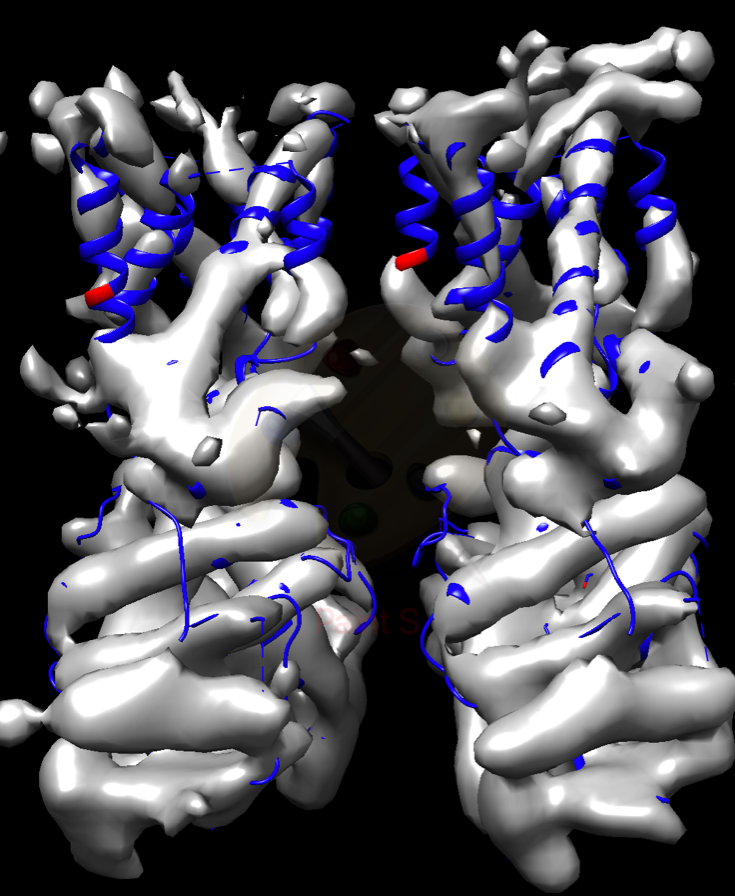
\includegraphics[width=0.9\textwidth]{real_map.png}
        \end{tikzfigure}
\end{minipage}
\begin{minipage}{0.209\textwidth}
{\Large Deep Simulation -cryoGAN}
        \begin{tikzfigure}
           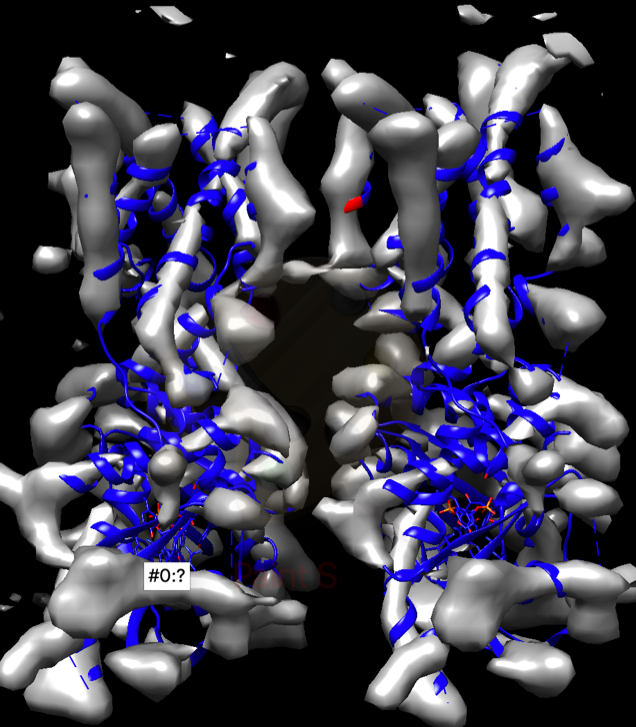
\includegraphics[width=0.9\textwidth]{gen_map.png}
        \end{tikzfigure}
\end{minipage}
    }
    \column{0.3}
    \block{7. Evaluation}{\begin{itemize}
	\item Visual inspection shows that the generated map has the features of an  experimental map.
	\item We trained an additional \textbf{ discriminator}  to distinguish between real and “fake” maps
	\item The REAL/SYM discriminator labels as real 41000 from 73000 test voxels from map

\end{itemize}}
        
	\note[
        targetoffsetx=-5.5cm, 
        targetoffsety=-9.5cm, 
        width=0.22\linewidth
        ]{e-mail: \textit{markroza@tauex.tau.ac.il}  }
    

    
\end{columns}
 
\begin{columns}
    \column{0.33}
    \block{8. VAE-GAN \cite{Wu}: Training VAE network to confuse the discriminator}
    {
        \begin{tikzfigure}
           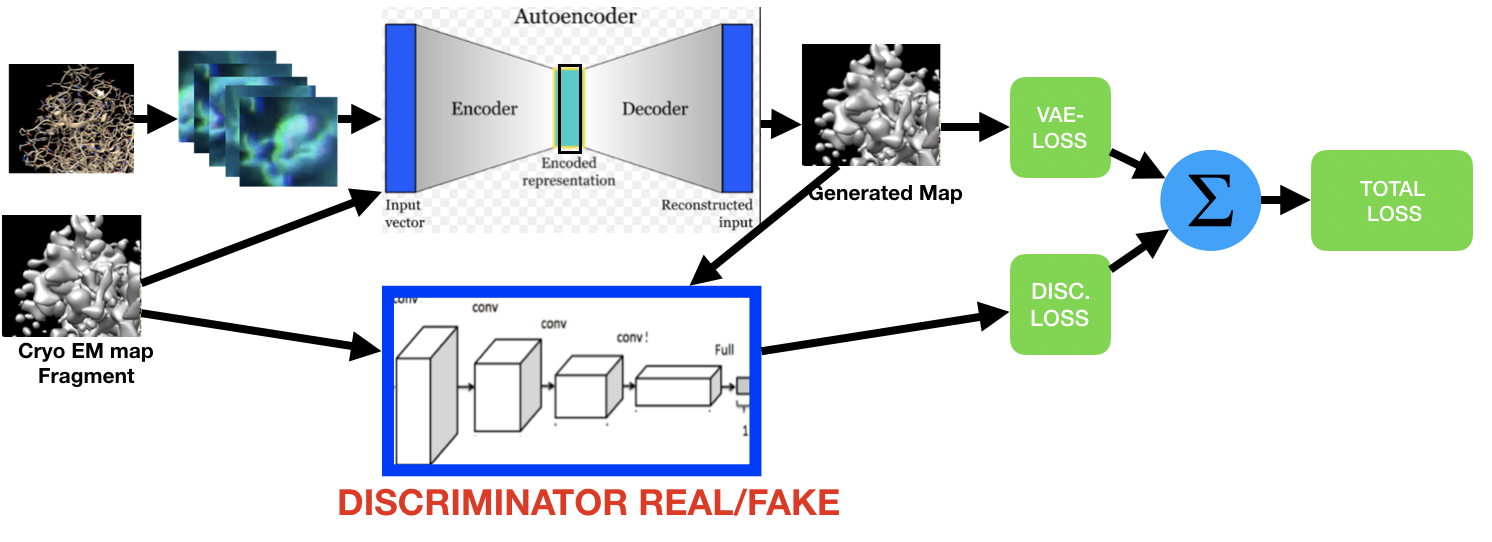
\includegraphics[width=0.28\textwidth]{vae-gan.png}
        \end{tikzfigure}
    }
    \column{0.4} 
    \block{}{{ \tiny
\bibliographystyle{abbrv}
 \bibliography{ref}
}}
    \column{0.25} 
    \block{Acknowledgments}{\textbf{Acknowledgments:}  This work has been supported in part by a fellowship from the Edmond J. Safra Center for Bioinformatics at Tel-Aviv Univesity, by Len Blavatnik and the Blavatnik Family Foundation ,and  by the I-CORE program of the Budgeting and Planning Commitee}
\end{columns}

\end{document}
